\section{Genetsko programiranje}
\emph{Genetsko programiranje} (\emph{GP}) je evolucijski algoritam koji do rješenja dolazi iterativno mjenjajući populaciju sve dok uvjet zaustavljanja nije zadovoljen (\cite{conv_gen_programming}).

Inspiraciju vuče iz prirode.
Algoritam počinje s nasumično nastalom populacijom koja se poboljšava kroz ograničen broj generacija.
Nastanak svake generacije započinje izborom jedinki (detaljno opisane u nastavku).
Izbor nije nasumičan niti determinističan, boljim jedinkama daje se prednost pri izboru no i one lošije mogu biti izabrane.
Nedeterminističnost izbora rezultira širem pretraživanju prostora rješenja, ne ograničenim samo na najbolje jedinke.
Iz jedinki nastaju nove kao rezultat genetskih operatora \emph{Križanja} i \emph{Mutacije}.
Ciklus se ponavlja sve dok jedna od dvije stvari nije zadovoljena:
\begin{itemize}
	\item{Dosegnut najveći broj iteracija ili evaluacija}
	\item{Postignuta željena preciznost rješenja (npr. $greska \leq 10^{-3}$})
\end{itemize}
Na kraju postupka, dobiveni model osim što se može koristiti u željenu svrhu, lako se može izučiti i interpretirati, jer za razliku od neuronskih mreža, način na koji ulaz postaje izlaz jasno je čitljiv. \\
Jednostavan primjer genetskog algoritma vidljiv je u pseudokodu ~\ref{alg:gp_example}

\begin{algorithm}
	\caption{Jednostavni genetski algoritam (\cite{wong2015evolutionary})}
	\label{alg:gp_example}
	\begin{algorithmic}
		\STATE $P(t)$: Roditeljska populacija u generaciji $t$
		\STATE $O(t)$: Populacija potomaka u generaciji $t$
		\STATE $P(t)=$ stvori\_pocetnu\_populaciju()
		\WHILE{uvjet zaustavljanja nije zadovoljen}
			\STATE $P^{'}(t) =$ izabrani roditelji iz $P(t)$
			\STATE $O(t + 1) =$ potomci nastali krizanjem jedinki iz $P^{'}(t)$
			\STATE $O(t + 1) = mutiraj\ O(t + 1)$
			\STATE $evaluiraj(O(t + 1))$
			\STATE $P(t + 1) = O(t + 1)$
			\STATE $t = t + 1$
		\ENDWHILE
	\end{algorithmic}
\end{algorithm}

\subsection{Jedinka populacije}
Jedinka populacije u genetskom algoritmu predstavlja jedno moguće rješenje na problem koji smo postavili.
Svaka jedinka je definirana s dvije stavke:
\begin{itemize}
	\item{Genotipom}
	\item{Načinom mapiranja genotipa u \emph{fenotip}}
\end{itemize}
Na najnižoj razini, svaka jedinka je jedan genotip. 
U praksi, genotip može biti prikazan na bilo koji način koji odgovara korisniku algoritma, no neke od najčešćih struktura su vektori brojeva, simbola ili bitova, fiksne ili varijabilne duljine, te stablaste strukture (\cite{naturally_selecting_algorithms}).
Korisnik koji koristi \emph{genetski algoritam} (GA) za pronalazak rješenja mora također definirati mapiranje $genotip \rightarrow fenotip$.
Genotipom možemo smatrati ono što koristi algoritam kako bi stvorio fenotip, dok je fenotip jedno od mogućih rješenja na problem koji rješavamo.
Što to znači?
Ukoliko je zadatak GA iz skupa točaka provesti simboličku regresiju $A\sin(Bx + C)$ gdje su $A$, $B$ i $C$ nepoznate varijable genotip bi se mogao prikazati kao vektor s broja s pomičnim zarezom.
Dalje, pravilo mapiranja genotipa u fenotip bi moglo biti da element na prvom mjestu odgovara vrijednosti koju pridajemo varijabli $A$ i tako dalje za varijable $B$ i $C$ (~\ref{fig:genotype_phenotype_map}).
Također, bitno je kvantificirati kvalitetu jedinke.
Ta mjera najčešće se naziva kondicija (\emph{eng. fitness}).
Sve jedinke populacije dobivaju kondiciju na temelju istog pravila kako bi bili međusobno usporedivi.
Jedinka s najvećom kondicijom smatra se najkvalitetnijom i najboljim rješenjem na problem koji se rješava.

\begin{figure}
	\caption{Mogućnosti spremanja i korištenja genotipa tijekom izvođenja genetskog algoritma}
	\begin{subfigure}[t]{0.45\textwidth}
		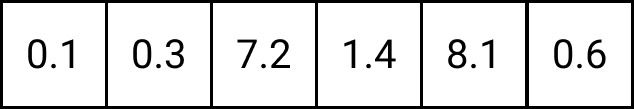
\includegraphics[width=\textwidth]{Illustrations/float_genotype.png}
		\caption{Genotip prikazan brojem s pomičnim zarezom}
	\end{subfigure}
	\hspace{\fill}
	\begin{subfigure}[t]{0.45\textwidth}
		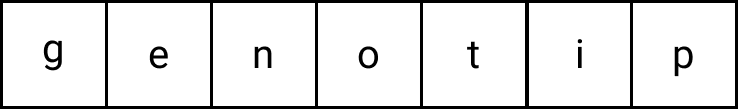
\includegraphics[width=\textwidth]{Illustrations/char_genotype.png}
		\caption{Genotip prikazan ascii znakovima}
	\end{subfigure}
	\label{fig:genotype_types}
\end{figure}

\begin{figure}
	\centering
	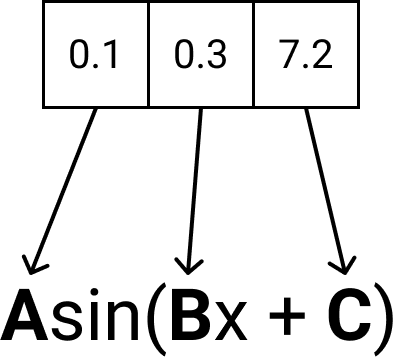
\includegraphics[width=0.4\linewidth]{Illustrations/genotype_phenotype_mapping.png}
	\caption{Primjer mapiranja genotipa u fenotip}
	\label{fig:genotype_phenotype_map}
\end{figure}

\subsection{Genetski operatori}
Genetski operatori pružaju osnovni mehanizam pretrage genetskog algoritma.
Za zadatak imaju stvarati nova rješenja uz efektivnu pretragu prostora rješenja.
Izvode se na primitivu jedinki, genotipu, te se nerjetko međusobno izvode u kombinaciji jer samostalno nisu uvijek efektivni.
U nastavku su opisane 2 osnovne vrste genetskih operatora, križanje i mutacija.

\subsubsection{Križanje}
Operator križanja u genetskom algoritmu oponaša reprodukciju u biološkom svijetu.
Od dvije jedinke stvara nove primjenjujući neko definirano pravilo kombinacije njihovih genotipa.
Križanje nije trivijalno kao na prvi pogled, te je usko ovisno o izboru strukture podataka s kojom definiramo genotip (~\cite{wong2015evolutionary}). \\
Na slici ~\ref{fig:crossover} prikazan je primjer jednog od operatora križanja koje ću detaljnije opisati u nastavku.

\begin{figure}
	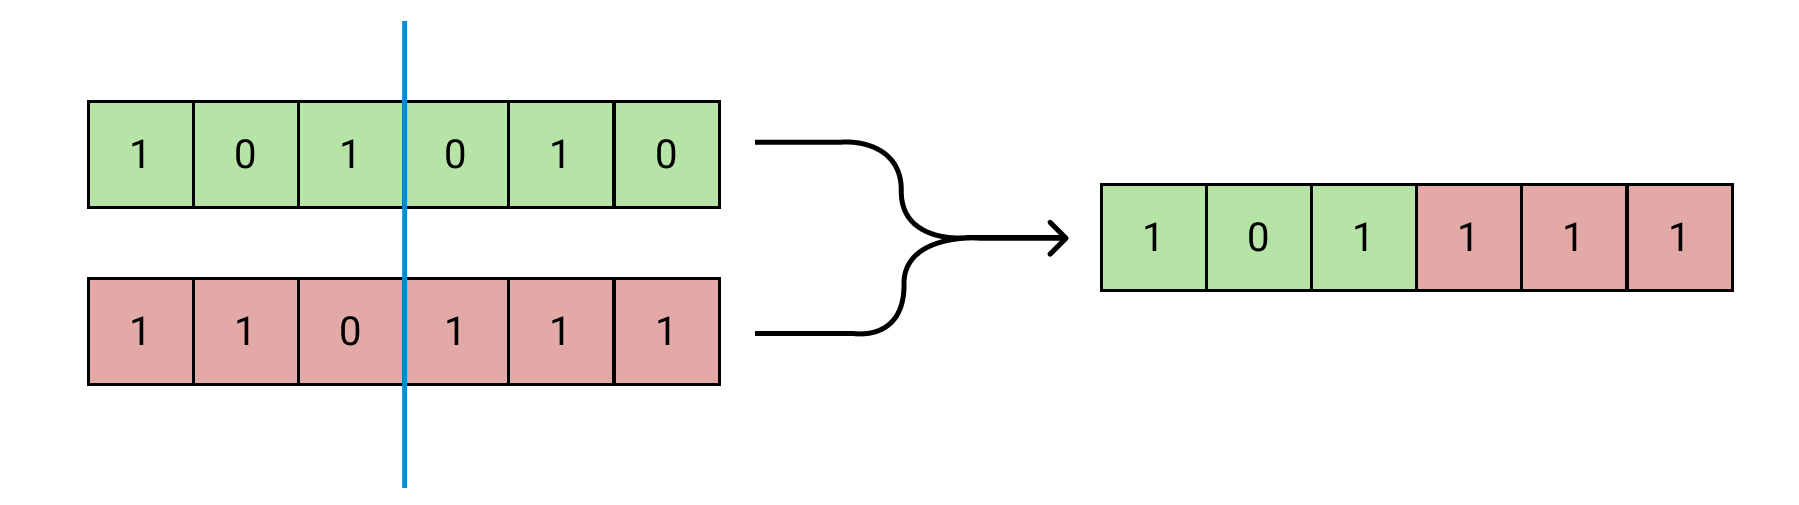
\includegraphics[width=\linewidth]{Illustrations/crossover.png}
	\caption{Jednostavni primjer rezultata primjene operatora križanja}
	\label{fig:crossover}
\end{figure}

\paragraph{Križanje u k točaka}
se koristi tako da se odabere $k$ nasumičnih točaka koje služe kao granica između kojih se uzimaju dijelovi dva različita genotipa.
Često se odabere $k = 1$ (primjer na slici ~\ref{fig:crossover}) zbog svoje jednostavnosti.
Ono što se često zamjera križanju u jednoj točki je pristranost poziciji genotipa.
To znači da će pri odabiru dva roditeljska genotipa $P_1$ i $P_2$ lijevi dio novonastalog genotipa uvijek pripasti pripadajućem dijelu $P_1$ a desni $P_2$.
Rješenje na taj problem, osim odabira $k > 1$, je stvaranje dva potomka koja se zatim evaluiraju, nakon čega se potomak koji se pokaže boljim prenosi u sljedeću generaciju populacije (ilustracija ~\ref{fig:position_bias}).

\begin{figure}
	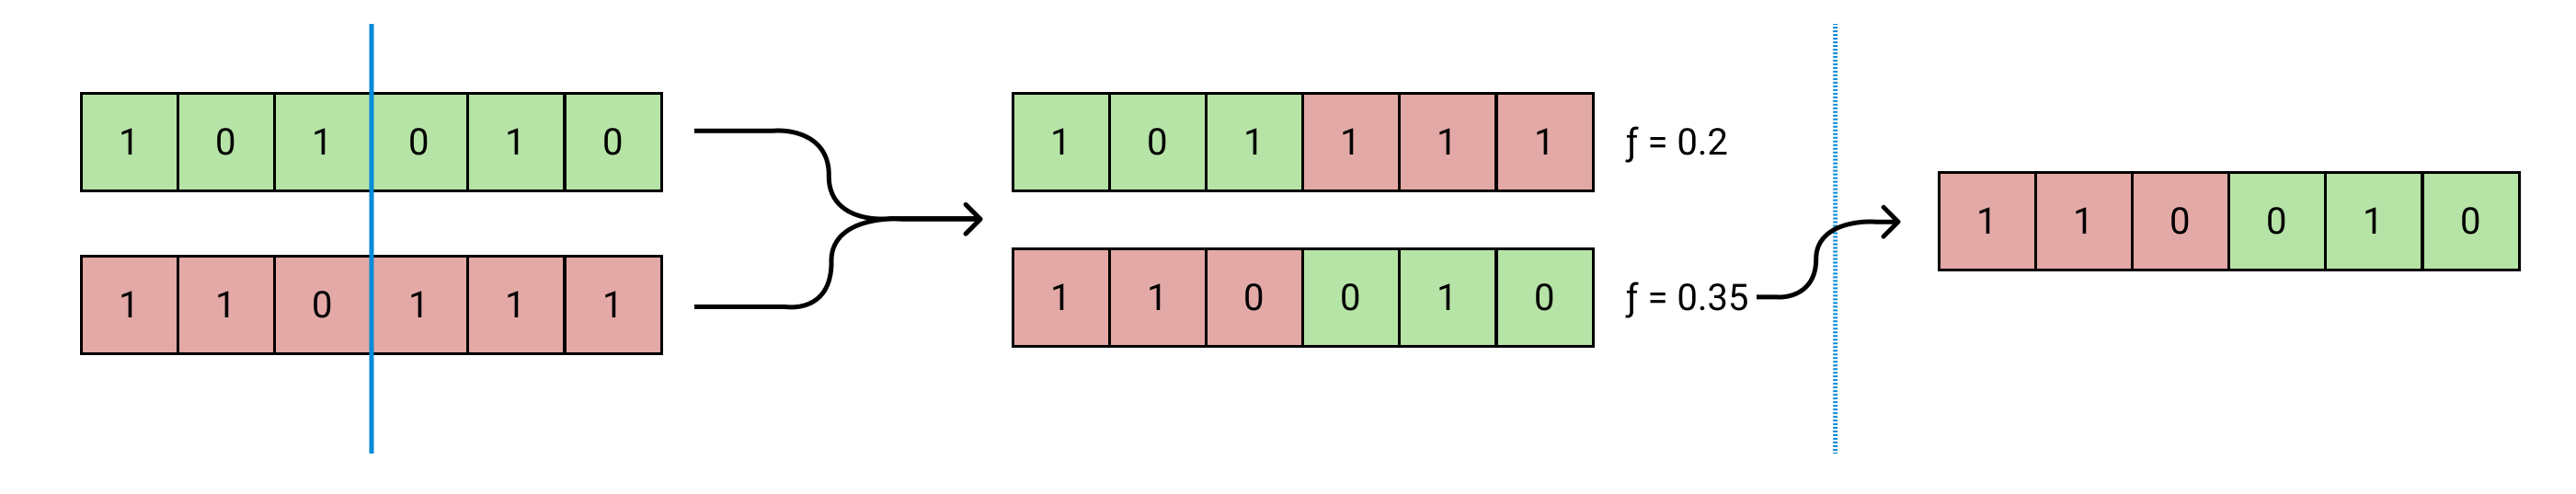
\includegraphics[width=\linewidth]{Illustrations/position_bias.png}
	\caption{Primjer rješavanja problema pristranosti pozicije}
	\label{fig:position_bias}
\end{figure}

\paragraph{Ujednačeno križanje (\emph{eng. Uniform crossover})}
tretira svaki gen u genotipu zasebno što osigurava da svaki roditeljski gen ima jednaku vjerojatnost da se prenese na novonastali genotip.
Postupak se može definirati kao:
\[
	O[n] = \left\{\begin{array}{lr}
			P_1[n], & \text{za } 0 \leq \alpha \leq 0.5 \\
			P_2[n] & \text{za } 0.5 < \alpha \leq 1
		\end{array}\right\}
\]
Također, grafički prikazano na ilustraciji ~\ref{fig:uniform_crossover}.

\begin{figure}
	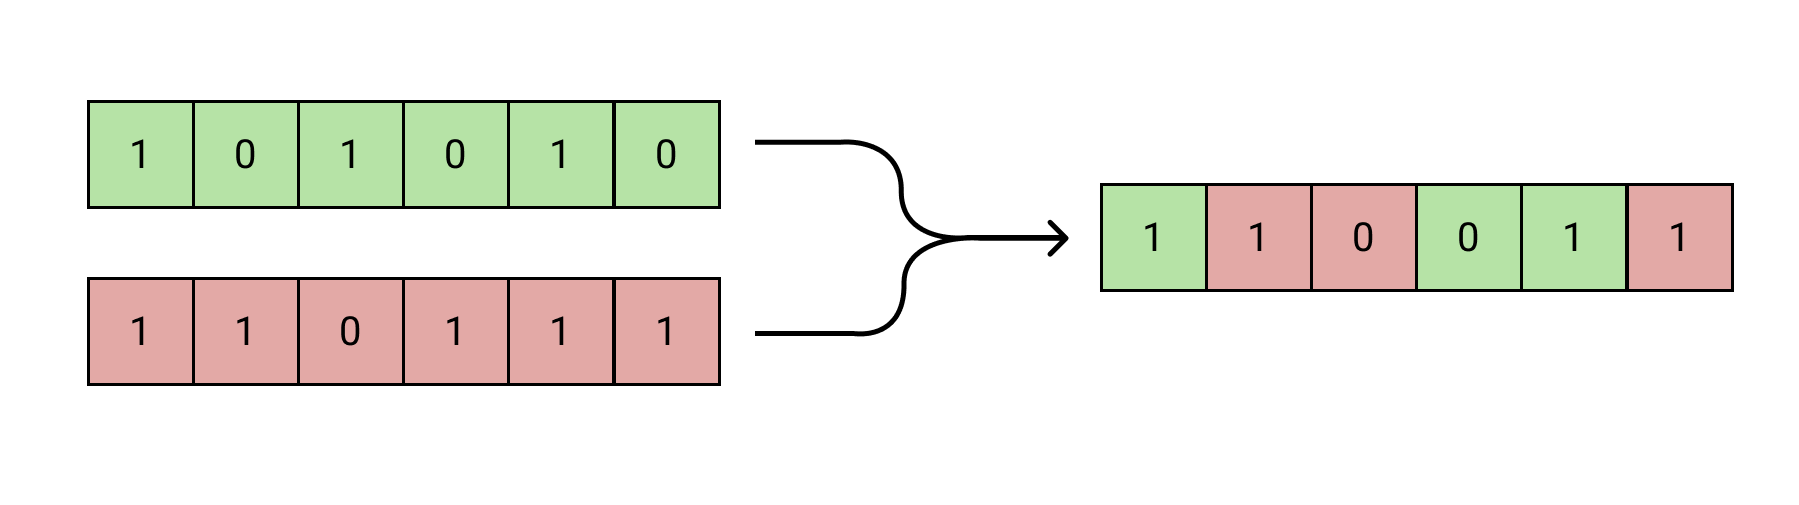
\includegraphics[width=\linewidth]{Illustrations/uniform_crossover.png}
	\caption{Rezultat primjene ujednačenog križanja}
	\label{fig:uniform_crossover}
\end{figure}

\subsubsection{Mutacija}
Analogno istoimenoj pojavi u biološkom svijetu, mutacija unosi male i nasumične promjene u genotip.
Primjena mutacije na genotip ne mora nužno promjeniti ni jedan gen, a može promjeniti i svaki.
Šansa za mutaciju se zadaje od strane korisnika i ne treba biti prevelika jer, u tom slučaju algoritam se svodi na nasumičnu pretragu.
U najviše slučajeva, vrijednost mutacije $\leq 5\%$ daje dobre rezultate.
Isto tako, vrijednost mutacije ne mora biti statična kroz cijeli algoritam.
Primjerice, u ranim iteracijama algoritma može biti korisno imati nešto veću vjerojatnost za mutaciju kako bi pretraživali veći prostor rješenja a u kasnijim iteracijama, kada smo nešto bliže rješenju, smanjiti tu vjerojatnost kako bismo manjim izmjenama došli do globalnog optimuma.
Razlog zbog kojeg se koristi mutacija je što pridonosi različitosti u populaciji.
Korištenje samo križanja potiče problem konvergencije u lokalnom minimumu, što se pokušava izbjeći unošenjem nasumičnih promjena tako potičući razliku između jedinki.
Imajući to na umu važno je napomenuti da se genetski algoritam može koristiti koristeći samo mutaciju.
Isto se ne može reći za križanje.
Pri rješavanju problema, ne moramo se ograničiti na jednu vrstu mutacije već se dodatna nasumičnost može unjeti korištenjem više vrsta mutacije odjednom.

\paragraph{Okretanje bitova (\emph{eng. Bit flip})} 
je mutacija koja je primjenjiva samo na genotipima opisanim kao vektor bitova \emph{npr.} $[1 0 0 1 0 1 1 0 1 1 1]$.
Uz zadani parametar $\alpha$, koji primjerice može biti $\alpha = \frac{1}{duljina\ vektora}$, svaki bit uz zadanu vjerojatnost negira, pretvarajući $0 \rightarrow 1$ i suprotno (ilustracija ~\ref{fig:bit_flip_mutation}).

\begin{figure}
	\centering
	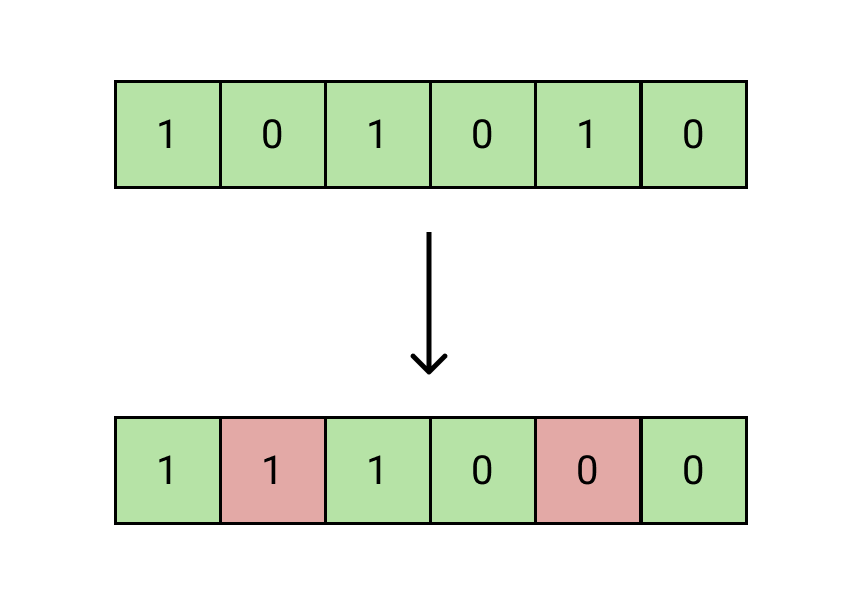
\includegraphics[width=0.5\linewidth]{Illustrations/bit_flip_mutation.png}
	\caption{Rezultat primjene mutacije okretanjem bitova}
	\label{fig:bit_flip_mutation}
\end{figure}

\paragraph{Ujednačeno mutiranje (\emph{eng. Uniform mutation})}
se koristi na genotipima opisanim cijelim brojevima ili brojevima s pomičnom točkom.
Svaki gen koji mutira mijenja u novu nasumičnu vrijednost unutar dozvoljene domene ukoliko ona postoji (ilustracija ~\ref{fig:uniform_mutation}).

\begin{figure}
	\centering
	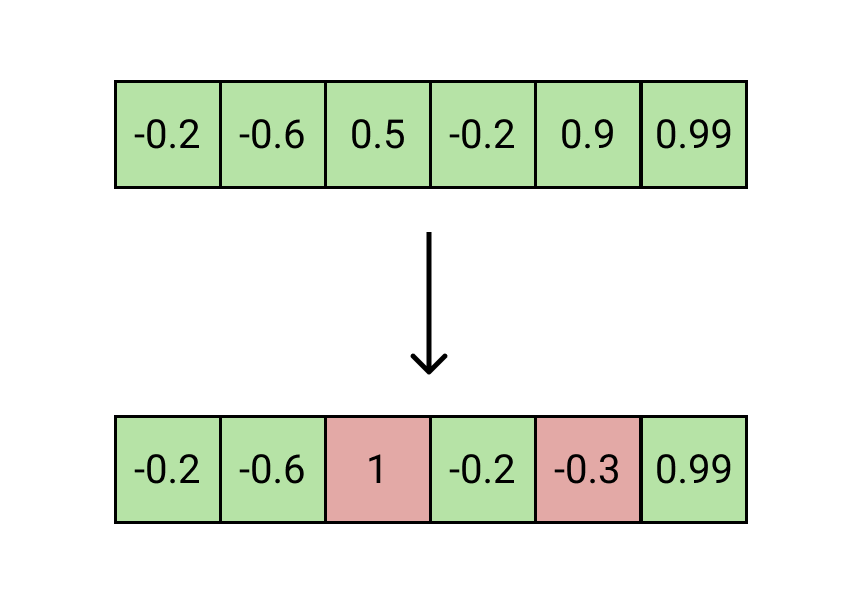
\includegraphics[width=0.5\linewidth]{Illustrations/uniform_mutation.png}
	\caption{Rezultat primjene ujednačene mutacije na genotip za čije gene vrijedi $gen \in [-1, 1]$}
	\label{fig:uniform_mutation}
\end{figure}

\paragraph{Mutiranje Gaussovim šumom}
osim nasumične varijable $\alpha$ koja predstavlja vjerojatnost da će gen biti mutiran, koristi i nasumičnu varijablu $X$, distribuiranu Gaussovom raspodjelom, odnosno $X \sim \mathcal{N}(\mu,\sigma^2)$ gdje $\mu$ srednja vrijednost, a $\sigma^2$ varijanca.
Svakom genu koji će biti mutiran pridodaje se šum $X$ (ilustracija ~\ref{fig:gaussian_mutation}).

\begin{figure}
	\centering
	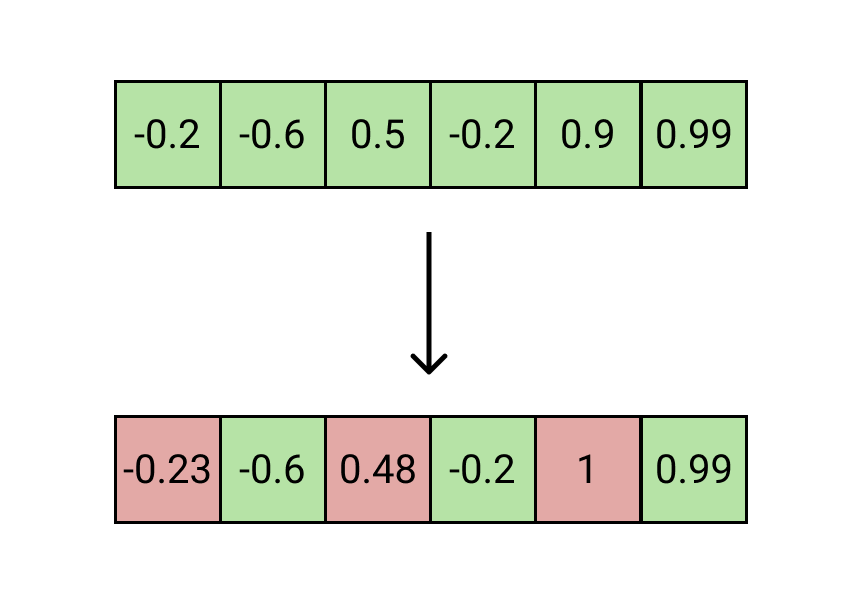
\includegraphics[width=0.5\linewidth]{Illustrations/gaussian_mutation.png}
	\caption{Rezultat primjene mutacije Gaussovim šumom}
	\label{fig:gaussian_mutation}
\end{figure}

\subsection{Elitizam}
Elitizam je broj najboljih jedinki koje se bez mutiranja prenose u sljedeću generaciju, osiguravajući preživljavanje najboljih jedinki (~\cite{elitism}).
Definira se cjelobrojnom vrijednosti $\in [0, broj\ jedinki\ u\ populaciji]$.
U slučaju da je vrijenost 0, ni jedna jedinka se ne prenosi.
Pretpostavka iza korištenja elitizma je da će nastati dobar balans između različitosti populacije uzrokovane križanjem i mutacijom potičući pretraživanje širokog prostora rješenja i konstantnog globalnog napretka uzrokovanog elitizmom.
Rezultat pretpostavke je brža i monotonija konvergencija ka globalnom optimumu.
Graf ~\ref{fig:elitism} prikazuje utjecaj elitizma pri optimizaciji strategije usmjeravanja podataka prenošenim bežičnom mrežom.

\begin{figure}
	\centering
	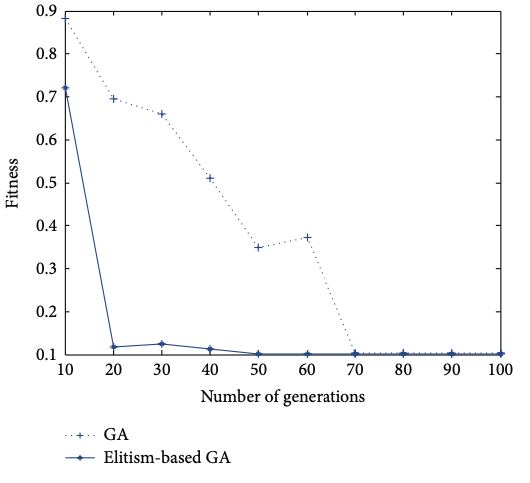
\includegraphics[width=0.7\linewidth]{SourcedGraphs/elitism_comparison.png}
	\caption{Usporedba izvođenja genetskog algoritma sa i bez elitizma pri rješavanju optimizacijskog problema}
	\label{fig:elitism}
\end{figure}


\subsection{Uvjet zaustavljanja}
Genetski algoritmi su posebno prikladni i efikasni u rješavanje problema s velikim prostorima pretrage te problemima gdje uobičajeni algoritmi ne bi bili polinomijalno učinkoviti (npr. NP-potpuni problemi) (~\cite{brassard1988algorithmics}).
Pripadanje u skupinu \emph{mekog računarstva} ne garantira potpuno precizna rješenja, već dovoljno precizna za samouvjereno donošenje zaključaka na kraju izvođenja.
Također, algoritam se izvodi kroz ograničeni broj koraka.
Postavlja se pitanje, kada zaustaviti koračanje, odnosno algoritam?
U praksi, najčešće se koriste sljedeća tri uvjeta zaustavljanja (~\cite{ga_stopping_criteria}):
\begin{itemize}
	\item Dosegnut najveći dozvoljeni broj generacija
	\item Dosegnut najveći dozvoljeni broj evaluacija kondicijske funkcije
	\item Dosegnuta željena preciznost
\end{itemize}
Ograničenje najvećeg dozvoljenog broja generacija i evaluacija kondicijske funkcije su statička ograničenja.
Je li uopće moguće precizno odrediti najbolje vrijednosti za statička ograničenja? \\
Slijepo postavljanje abnormalno velikih vrijednosti te postepeno smanjivanje kroz sljedeća pokretanja algoritma je iznimno neučinkovito.
Potrebno je određeno znanje o problemu kako bi se postavila barem približno precizna ograničenja na duljinu pretrage prostora rješenja. \\
Dosegnuta željena preciznost je dinamičko ograničenje koje se može i ne mora doseći u bilo kojem trenutku.
To znači da za neki problem, za koji smo postavili ograničenje na npr. najviše $100$ generacija, možemo doseći uvjet zaustavljanja npr. grešku $\leq 10^{-3}$ već nakon desetak generacija ako je problem jednostavan ili smo slučajno dobili početnu točku blisku globalnom optimumu.
Analogno tome, zapinjanje u lokalnom optimumu može izazvati istek statičkih ograničenja bez postizanja željene preciznosti. \\
Znači li spomenuto da je dostizanje željene preciznosti najbolje mjerilo kvalitete dobivenog modela? \\
U kontekstu \emph{strojnog učenja}, čemu pripada i genetsko programiranje, često se spominju različiti skupovi podataka. \\
Razlikujemo tri skupa (~\cite{datasets}):

\paragraph{Skup za trening}
su podaci na temelju kojih se model \emph{uči} uspoređujući svoje izlaze sa željenim iz skupa.

\paragraph{Skup za validaciju} 
je objektivniji skup podataka na kojima se model nikad ne uči.
S obzirom na svojstvo učenja da će pokušati najbolje preslikati ulaze na izlaze što sličnije željenim iz skupa za trening lako može doći do \emph{pretreniranja}.
S tim na umu, validacijski skup je objektivnije mjerilo kvalitete modela.

\paragraph{Testni skup}
su podaci koji se prezentiraju konačnom modelu.
Odvajaju se od cjelokupnog skupa podataka na samom početku eksperimenta te su rezervirani za konačne modele koji se žele daljnije ispitati.
Imitiraju podatke i situacije iz stvarnog svijeta jer kako su podaci odvojeni na samom početku, model ih nikad nije vidio.
Slično validacijskom skupu s razlikom da se u ni jednoj točki postupka treniranja podaci iz testnog skupa ne prikažu modelu. \\

Spomenuti skupovi se nadovezuju na svojstvo algoritma da će kroz vrijeme samo preciznije svoje izlaze približavati onima na kojima se trenira dosežući pritom fazu pretreniranja.
Graf ~\ref{fig:train_test_loss} prikazuje ovisnost odstupanja na različitim skupovima podataka te optimalnu točku s najboljim objektivnim modelom.
Područje lijevo od označenog trenutka je vrijeme tijekom kojeg je model uz stalno učenje bio objektivan. 
Desno od trenutka je nastupilo pretreniranje.
Model sve bolje preslikava ulaze onima iz skupa za trening, no sve ostalo postaje nepreciznije.
Graf ~\ref{fig:overfitting} Prikazuje rad objektivnog i pretreniranog modela.

\begin{figure}
	\caption{Grafički prikaz odstupanja kroz iteracije na trening i validacijskom skupu podataka te prikaz rada pretreniranog modela}
	\begin{subfigure}[t]{0.48\textwidth}
		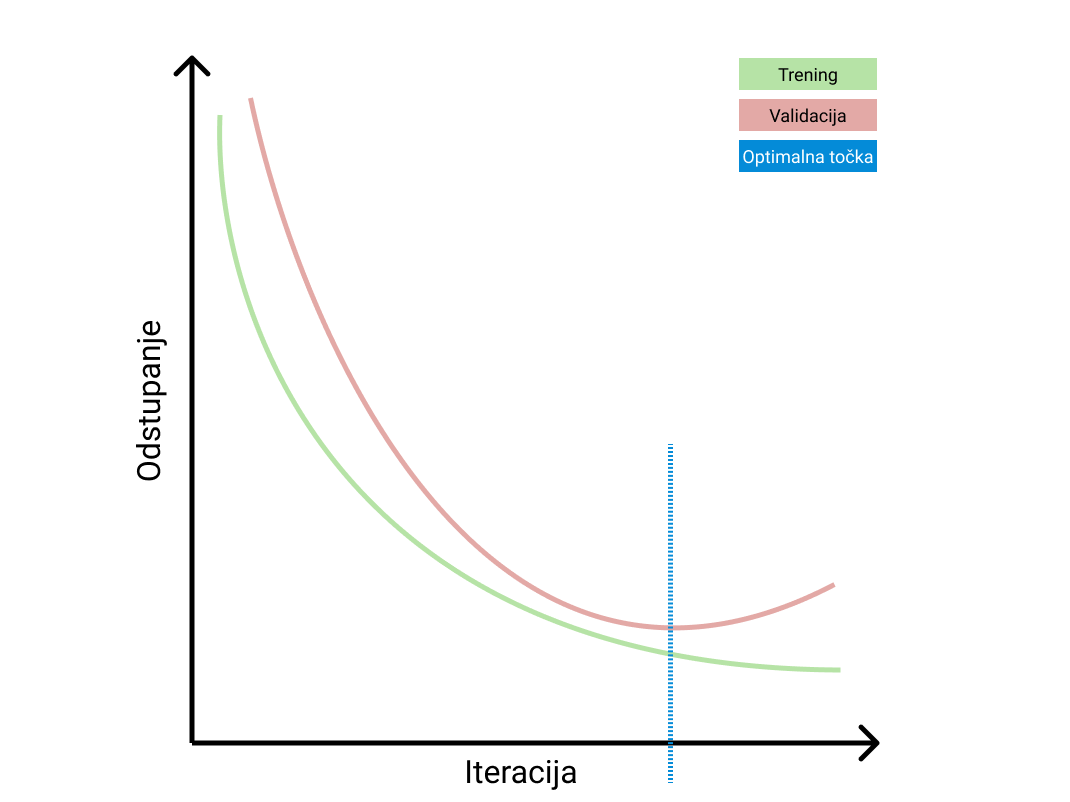
\includegraphics[width=\textwidth]{Illustrations/train_test_loss.png}
		\caption{Odstupanje na različitim skupovima podataka kroz iteracije}
		\label{fig:train_test_loss}
	\end{subfigure}
	\hspace{\fill}
	\begin{subfigure}[t]{0.48\textwidth}
		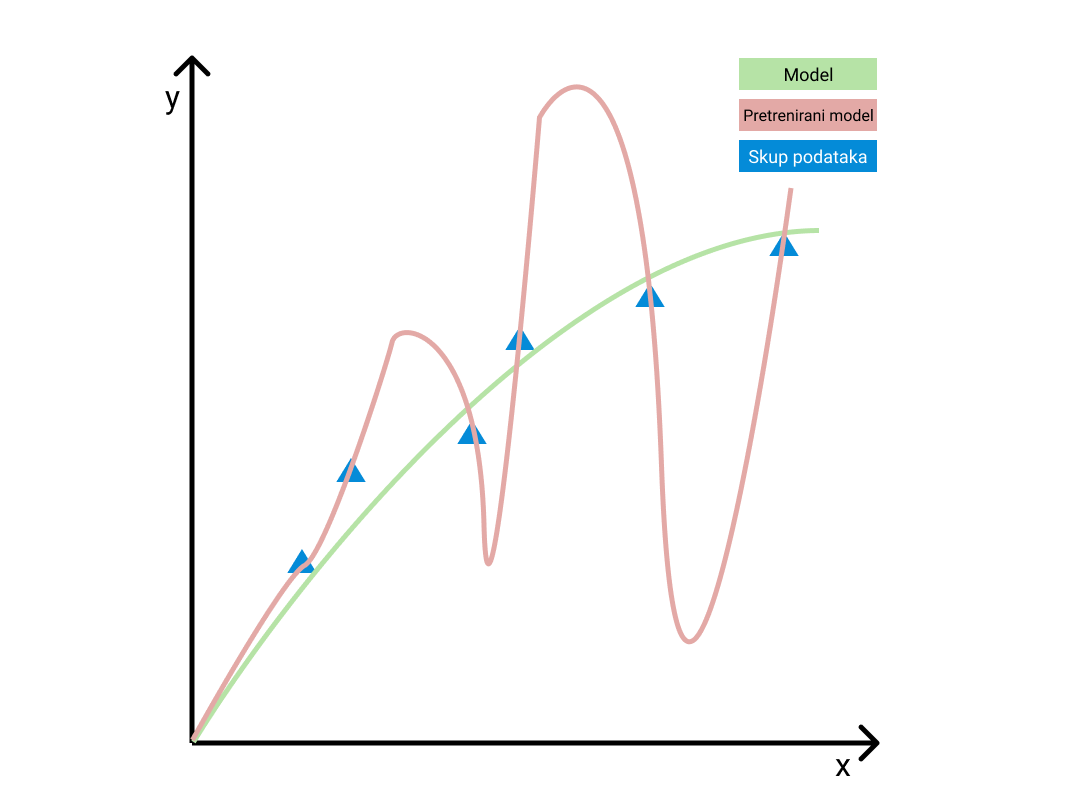
\includegraphics[width=\textwidth]{Illustrations/overtraining.png}
		\caption{Rad objektivnog i pretreniranog modela}
		\label{fig:overfitting}
	\end{subfigure}
\end{figure}

Iz priloženog je vidljivo kako tema uvjeta zaustavljanja nije jednostavna kao što se na prvu čini te postoji puno parametara koji uvjetuju koji model uzeti.
~\cite{ga_stopping_criteria} naglašava da korištenje isključivo statičkih ograničenja ne garantira dobre rezultate.
Dinamička provjera sa drugim skupovima podataka je pouzdana i provjerena metoda uz manu što znatno utječe na vrijeme izvođenja algoritma.
~\cite{fuzzy_logic} ispituju i predlažu korištenje meke logike kako bi definirali uvjet zaustavljanja.
Samo pogađanje i pretpostavka dobrih parametara je iznimno kompliciran problem koji se pojavljuje i prije pokretanja samog eksperimenta.
Također, s obzirom na rast računalne moći i na trenutne trendove (~\cite{ga_stopping_criteria}), adaptivni i dinamički uvjeti zaustavljanja su višestruko isplativi za korištenje tijekom rješavanja problema.

% TODO Tu nastavi kako treba imati train/val/test i onda gledati ako se 2 koraka pogorska val kvaliteta blaabla
% TODO Navedi uvjet zaustavljanja u kontekstu validacijskog skupa podataka
